% Drawing 154/09-7 -- folder 154, batch 09, archive page 171 (PDF page 172).
% Transcription: dessins en couleur et au crayon. En haut à gauche, une croix vert clair et un croisement orange sur une droite vert clair, une droite en tirets au-dessus. Au milieu, un grand cercle au crayon marqué de quatre arcs bleus et de flèches, et à l'intérieur un disque bordé de vert clair traversé de pseudo-droites noires, numérotées au bord $0$, $1$, $2$, $3$, …, $9$ d'un côté et $0'$, …, $9'$ de l'autre. En haut à droite, un grand disque traversé de pseudo-droites orange, triangles coloriés en jaune, avec au bord les numéros $1$, $2$, $3$, $1'$, $2'$, $3'$, $5$, $6'$, $8'$, $9$ et une flèche. En bas, un faisceau de droites orange et vert clair qui se tordent autour d'un croisement numéroté $1\,2\,3$ et $3\,2\,1$, avec une flèche ; un petit disque dont le bord est vert foncé sur une moitié et vert clair sur l'autre, numéroté $9$, $0$, $1$, $2$, $3$, $4$, … et $9'$, $8'$, …, $0'$, $1'$, $2'$, $3'$ ; enfin un nœud de pseudo-droites rouges serrées autour d'un segment noir hachuré, numérotées $1$, $2$, $3$. Les suites suivantes sont écrites entre les dessins
% Kind: crossings on lines; pencil circle with blue arcs round a disk with numbered rim; large orange disk with yellow sectors; numbered sequences; braids. Method 2 (schematic redraw from the facsimile). Status: partial.
% Notes: Colour and pencil drawings, read from the page view. Top left, a light green cross, and an orange crossing on a light green line with a dashed line above. Middle, a large pencil circle marked by four blue arcs and arrows, holding a disk with yellow-green rim crossed by black curves, its rim points numbered 0 ... 9 and 0' ... 9' (numbers not reproduced). Top right, a large disk crossed by orange pseudolines, sectors coloured yellow (drawn as wedges). The digit sequences with braces (« 321045678 ... ») are given only by their place; bottom: crossings on a line, a small disk with numbered rim, and a braid of red curves round a dark band. Strands schematic. Still differs from the facsimile: Middle, a large pencil circle marked by four blue arcs and arrows, holding a disk with yellow-green rim crossed by black curves, its rim points numbered 0 ... 9 and 0' ... 9' (numbers not reproduced). Strands schematic. 7 coloured or hatched triangle(s) are placed schematically and are not bounded by the strands that bound them on the page.
% Coordinates: 1 unit = 1 mm = 1/100 of the crop width (bbox in page fractions: [0.175, 0.079, 0.873, 0.505]).
% Redrawn by Claude (claude-opus-5-5), issue #73, 2026-11-07; not checked by a human; not compiled (no TeX in the session).
% Revised by Claude (claude-opus-5-5) 2026-11-09 (issue #128) after Michel's check: vertices snapped to exact intersections (drawn points on their lines, meeting ends on the stroke they meet, near-concurrent lines through one computed point, curve ends on their rim); labels at \small as in folder 80 batch 3. Status: partial.
% Rights: reproduces part of the work -- behind RENDER_TRANSCRIPTS, never published by itself.
\documentclass[tikz,border=3pt]{standalone}
\usepackage{amsmath,amssymb}
\usetikzlibrary{patterns,arrows.meta}
\tikzset{Or/.style={orange!90!black}, Ye/.style={yellow!80!orange}, Lg/.style={green!60!black!70}, Dg/.style={green!45!black}, Br/.style={brown!80!black}, Rd/.style={red!85!black}, Bl/.style={blue!70!black}, Gy/.style={black!40}, pencil/.style={black!45}, struck/.style={black!35}, mark/.style={circle,draw,inner sep=1.3pt}, pt/.style={circle,fill,inner sep=0.9pt}, opt/.style={circle,draw,fill=white,inner sep=1.1pt}}
\begin{document}
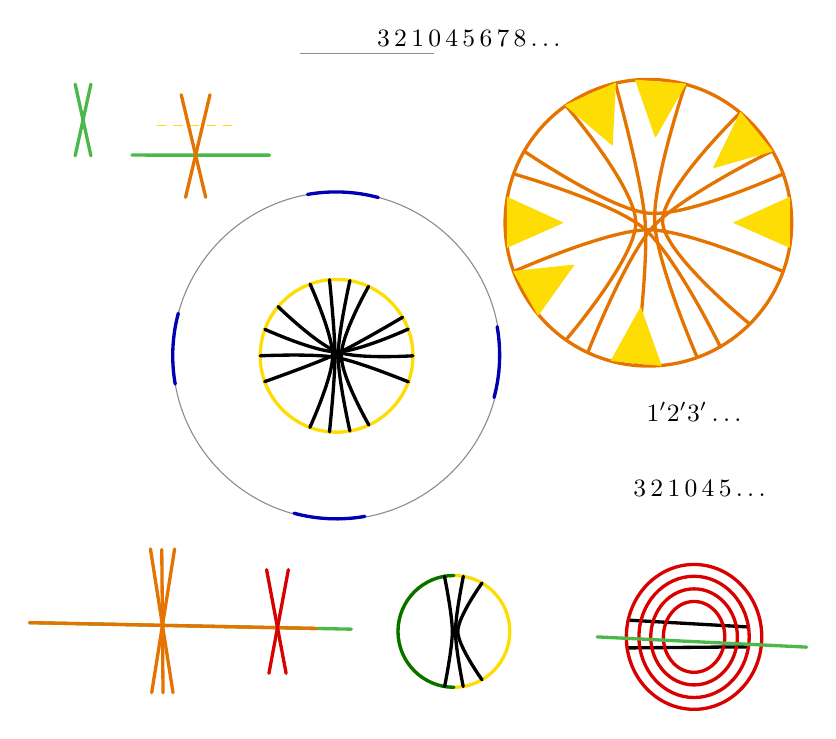
\begin{tikzpicture}[x=1mm,y=1mm,line cap=round,line join=round,font=\scriptsize]
\draw[Lg,very thick] (7.1,-7.1) -- (9.1,-16.2);
\draw[Lg,very thick] (9.1,-7.1) -- (7.1,-16.2);
\draw[Lg,very thick] (14.3,-16.11) -- (31.8,-16.12);
\draw[Ye,dashed] (17.5,-12.3) -- (27.9,-12.3);
\draw[Or,very thick] (20.57,-8.45) -- (23.68,-21.48);
\draw[Or,very thick] (24.22,-8.45) -- (21.12,-21.48);
\draw[pencil] (40.3,-41.6) circle[radius=20.8];
\draw[Bl,very thick] (45.6,-21.5) arc[start angle=75, end angle=100, x radius=20.8, y radius=20.8];
\draw[Bl,very thick] (20.2,-36.2) arc[start angle=165, end angle=190, x radius=20.8, y radius=20.8];
\draw[Bl,very thick] (34.9,-61.6) arc[start angle=255, end angle=280, x radius=20.8, y radius=20.8];
\draw[Bl,very thick] (60.3,-46.9) arc[start angle=345, end angle=370, x radius=20.8, y radius=20.8];
\draw[Ye,very thick] (40.3,-41.6) circle[radius=9.7];
\draw[very thick] plot[smooth, tension=0.55] coordinates {(36.94,-32.5) (39.8,-41.6) (36.91,-50.69)};
\draw[very thick] plot[smooth, tension=0.55] coordinates {(39.4,-31.94) (40.1,-41.6) (39.4,-51.26)};
\draw[very thick] plot[smooth, tension=0.55] coordinates {(41.99,-32.05) (40.5,-41.6) (41.99,-51.15)};
\draw[very thick] plot[smooth, tension=0.55] coordinates {(44.36,-32.79) (40.9,-41.6) (44.4,-50.39)};
\draw[very thick] plot[smooth, tension=0.55] coordinates {(32.87,-35.36) (40.4,-41.1) (50,-41.6)};
\draw[very thick] plot[smooth, tension=0.55] coordinates {(31.2,-38.24) (40.3,-41.1) (49.39,-38.21)};
\draw[very thick] plot[smooth, tension=0.55] coordinates {(30.6,-41.6) (40.2,-41.8) (49.42,-44.91)};
\draw[very thick] plot[smooth, tension=0.55] coordinates {(31.17,-44.88) (40.2,-41.4) (48.68,-36.71)};
\draw[Or,very thick] (79.9,-24.7) circle[radius=18.2];
\draw[Or,very thick] plot[smooth, tension=0.55] coordinates {(75.7,-7) (79.5,-24.7) (78.3,-42.83)};
\draw[Or,very thick] plot[smooth, tension=0.55] coordinates {(84.6,-7.1) (80.7,-24.6) (86.1,-41.81)};
\draw[Or,very thick] plot[smooth, tension=0.55] coordinates {(69.4,-9.8) (78.3,-24.7) (69.42,-39.58)};
\draw[Or,very thick] plot[smooth, tension=0.55] coordinates {(91.6,-10.7) (81.7,-24.6) (92.77,-37.57)};
\draw[Or,very thick] plot[smooth, tension=0.55] coordinates {(64.13,-15.62) (80,-23.5) (97.01,-18.5)};
\draw[Or,very thick] plot[smooth, tension=0.55] coordinates {(62.8,-30.9) (79.9,-25.6) (97.01,-30.9)};
\draw[Or,very thick] plot[smooth, tension=0.55] coordinates {(95.6,-15.6) (80.5,-25.2) (72.2,-41.19)};
\draw[Or,very thick] plot[smooth, tension=0.55] coordinates {(62.79,-18.5) (79.3,-25.4) (89.03,-40.45)};
\draw[Ye] (75.7,-7) -- (69.4,-9.8) -- (75.3,-14.8) -- cycle;
\fill[pattern=north east lines,Ye] (75.7,-7) -- (69.4,-9.8) -- (75.3,-14.8) -- cycle;
\draw[Ye] (84.6,-7.1) -- (78.3,-6.6) -- (80.8,-13.8) -- cycle;
\fill[pattern=north east lines,Ye] (84.6,-7.1) -- (78.3,-6.6) -- (80.8,-13.8) -- cycle;
\draw[Ye] (62,-21.5) -- (62,-27.8) -- (69,-24.7) -- cycle;
\fill[pattern=north east lines,Ye] (62,-21.5) -- (62,-27.8) -- (69,-24.7) -- cycle;
\draw[Ye] (97.8,-27.8) -- (97.8,-21.5) -- (90.8,-24.7) -- cycle;
\fill[pattern=north east lines,Ye] (97.8,-27.8) -- (97.8,-21.5) -- (90.8,-24.7) -- cycle;
\draw[Ye] (62.8,-30.9) -- (65.9,-36.4) -- (70.4,-30.1) -- cycle;
\fill[pattern=north east lines,Ye] (62.8,-30.9) -- (65.9,-36.4) -- (70.4,-30.1) -- cycle;
\draw[Ye] (75.2,-42.2) -- (81.5,-42.8) -- (78.9,-35.5) -- cycle;
\fill[pattern=north east lines,Ye] (75.2,-42.2) -- (81.5,-42.8) -- (78.9,-35.5) -- cycle;
\draw[Ye] (95.6,-15.6) -- (91.6,-10.7) -- (88.2,-17.7) -- cycle;
\fill[pattern=north east lines,Ye] (95.6,-15.6) -- (91.6,-10.7) -- (88.2,-17.7) -- cycle;
\draw[pencil] (35.7,-3.2) -- (52.6,-3.2);
\node[inner sep=1pt] at (57.1,-1.3) {\small $3\,2\,1\,0\,4\,5\,6\,7\,8\ldots$};
\node[inner sep=1pt] at (85.7,-48.7) {\small $1'2'3'\ldots$};
\node[inner sep=1pt] at (86.4,-58.4) {\small $3\,2\,1\,0\,4\,5\ldots$};
\draw[Lg,very thick] (1.28,-75.49) -- (42.18,-76.32);
\draw[Or,very thick] (1.31,-75.49) -- (37.72,-76.23);
\draw[Or,very thick] (16.66,-66.12) -- (19.53,-84.39);
\draw[Or,very thick] (19.73,-66.14) -- (16.82,-84.39);
\draw[Or,very thick] (18.1,-66.2) -- (18.26,-84.4);
\draw[Rd,very thick] (31.41,-68.76) -- (33.89,-81.92);
\draw[Rd,very thick] (34.18,-68.76) -- (31.71,-81.92);
\draw[Ye,very thick] (55.2,-76.6) circle[radius=7.1];
\draw[Dg,very thick] (55.2,-69.5) arc[start angle=90, end angle=270, x radius=7.1, y radius=7.1];
\draw[very thick] plot[smooth, tension=0.55] coordinates {(56.4,-69.6) (55.4,-76.6) (56.38,-83.6)};
\draw[very thick] plot[smooth, tension=0.55] coordinates {(58.77,-70.46) (55.7,-76.6) (58.77,-82.74)};
\draw[very thick] plot[smooth, tension=0.55] coordinates {(54,-69.6) (55,-76.6) (54.02,-83.6)};
\draw[very thick] (77.33,-75.17) -- (92.61,-76.04);
\draw[very thick] (77.2,-78.7) -- (92.61,-78.56);
\draw[Rd,very thick] (85.7,-77.3) ellipse[x radius=3.9, y radius=4.5];
\draw[Rd,very thick] (85.7,-77.3) ellipse[x radius=5.5, y radius=6.1];
\draw[Rd,very thick] (85.7,-77.3) ellipse[x radius=7, y radius=7.7];
\draw[Rd,very thick] (85.7,-77.3) ellipse[x radius=8.6, y radius=9.2];
\draw[Lg,very thick] (73.4,-77.3) -- (100,-78.6);
\end{tikzpicture}
\end{document}
